\documentclass{tikzposter}
\tikzposterlatexaffectionproofoff

\usepackage{hyperref}
\usepackage{doi}
\usepackage{qrcode}

\makeatletter
\renewcommand\TP@maketitle{%
   \begin{minipage}{0.7\linewidth}
    \color{titlefgcolor}
    {\bfseries \Huge \sc \@title \par}
    \vspace*{1em}
    {\huge \@author \par}
    \vspace*{1em}
    {\LARGE \@institute}
  \end{minipage}
  \hfill
  \begin{minipage}{0.3\linewidth}
     \centering
     \begin{tikzpicture}
       \begin{scope}[scale=0.12, y={(0,-1)}]
         \input{uoa.tex}
       \end{scope}
     \end{tikzpicture}
  \end{minipage}
}
\makeatother

\title{\parbox{\linewidth}{Estimating Mutation Parameters and Population History\\Simultaneously from Temporally-Spaced Genome Data}}
\author{\underline{Arman Bilge}, Tanja Stadler, Matthew Kearse, and Alexei J. Drummond}
\institute{\Large email: \href{mailto:abil933@aucklanduni.ac.nz}{\texttt{abil933@aucklanduni.ac.nz}}}

\defineblockstyle{MySlide}{
  titlewidthscale=1, bodywidthscale=1, titleleft,
  titleoffsetx=0pt, titleoffsety=0pt, bodyoffsetx=0pt, bodyoffsety=0pt,
  bodyverticalshift=0pt, roundedcorners=0, linewidth=0pt, titleinnersep=1cm,
  bodyinnersep=1cm
}{
  \ifBlockHasTitle%
    \draw[draw=none, left color=blocktitlebgcolor, right color=blocktitlebgcolor]
       (blocktitle.south west) rectangle (blocktitle.north east);
  \fi%
  \draw[draw=none, fill=blockbodybgcolor] %
    (blockbody.north west) [rounded corners=30] -- (blockbody.south west) --
    (blockbody.south east) [rounded corners=0]-- (blockbody.north east) -- cycle;
}

\usetheme{Autumn}
\usecolorstyle{Russia}
\definecolor{uoanavy}{RGB}{0,60,127}
\colorlet{titlebgcolor}{uoanavy}
\colorlet{blocktitlebgcolor}{uoanavy}
\useblockstyle{MySlide}
\renewcommand{\familydefault}{\sfdefault}
\usepackage{sfmath}

\usepackage{multicol}
\usepackage{enumitem}
\setlist[itemize]{label=$\triangleright$, labelsep=12pt}

\usepackage{pgfplots}
\pgfplotsset{
  /pgfplots/xlabel near ticks/.style={
     /pgfplots/every axis x label/.style={
        at={(ticklabel cs:0.5)},anchor=near ticklabel
     }
  },
  /pgfplots/ylabel near ticks/.style={
     /pgfplots/every axis y label/.style={
        at={(ticklabel cs:0.5)},rotate=90,anchor=near ticklabel}
     }
  }

\usepackage{amsmath}
\usepackage{amsfonts}

\usepackage[none]{hyphenat}
\frenchspacing

\begin{document}

  \maketitle

  \begin{columns}

    \column{0.5}

    \block{Motivation and Primary Challenges}{
      \flushleft
      \begin{itemize}
        \item Very feasible to sequence entire genomes
        \item More recently, even possible to recover \textbf{ancient genomes}
        \item \textbf{Temporally-spaced genome data}
        \item Opportunity to do \textbf{inference previously only possible for fast-evolving organisms} \\ (e.g., viruses)
        \begin{multicols*}{2}
          \begin{itemize}
          \item \textbf{mutation rate}
          \item \textbf{population size} through time
          \end{itemize}
        \end{multicols*}
        \end{itemize}
        \textbf{But\ldots}
        \begin{multicols*}{2}
          \begin{itemize}
            \item Difficult to phase diploid genomes
            \item Recombination
          \end{itemize}
        \end{multicols*}
        \begin{itemize}
        \item \textbf{Low coverage and sequencing error}, especially for ancient genomes
        \item \textbf{Cannot use existing Bayesian phylogenetic methods}
      \end{itemize}
    }

    \block{Sequencing Depth and Error}{

      \flushleft

      \begin{multicols*}{2}
        \setlength{\columnsep}{8pt}
        \begin{itemize}
          \item Assume that all individuals have \textbf{about same number of SNPs}
          \item Average sequencing depth of sample is \textbf{correlated} with observed SNPs
          \item Our dataset approaches complete SNP recovery at \textbf{22x coverage}
          \item Ancient genomes are sequenced at lower depth and thus \textbf{missing many SNPs}
          \item Leads to \textbf{systematic bias} in estimates
        \end{itemize}
        \vfill
        \null
        \columnbreak

        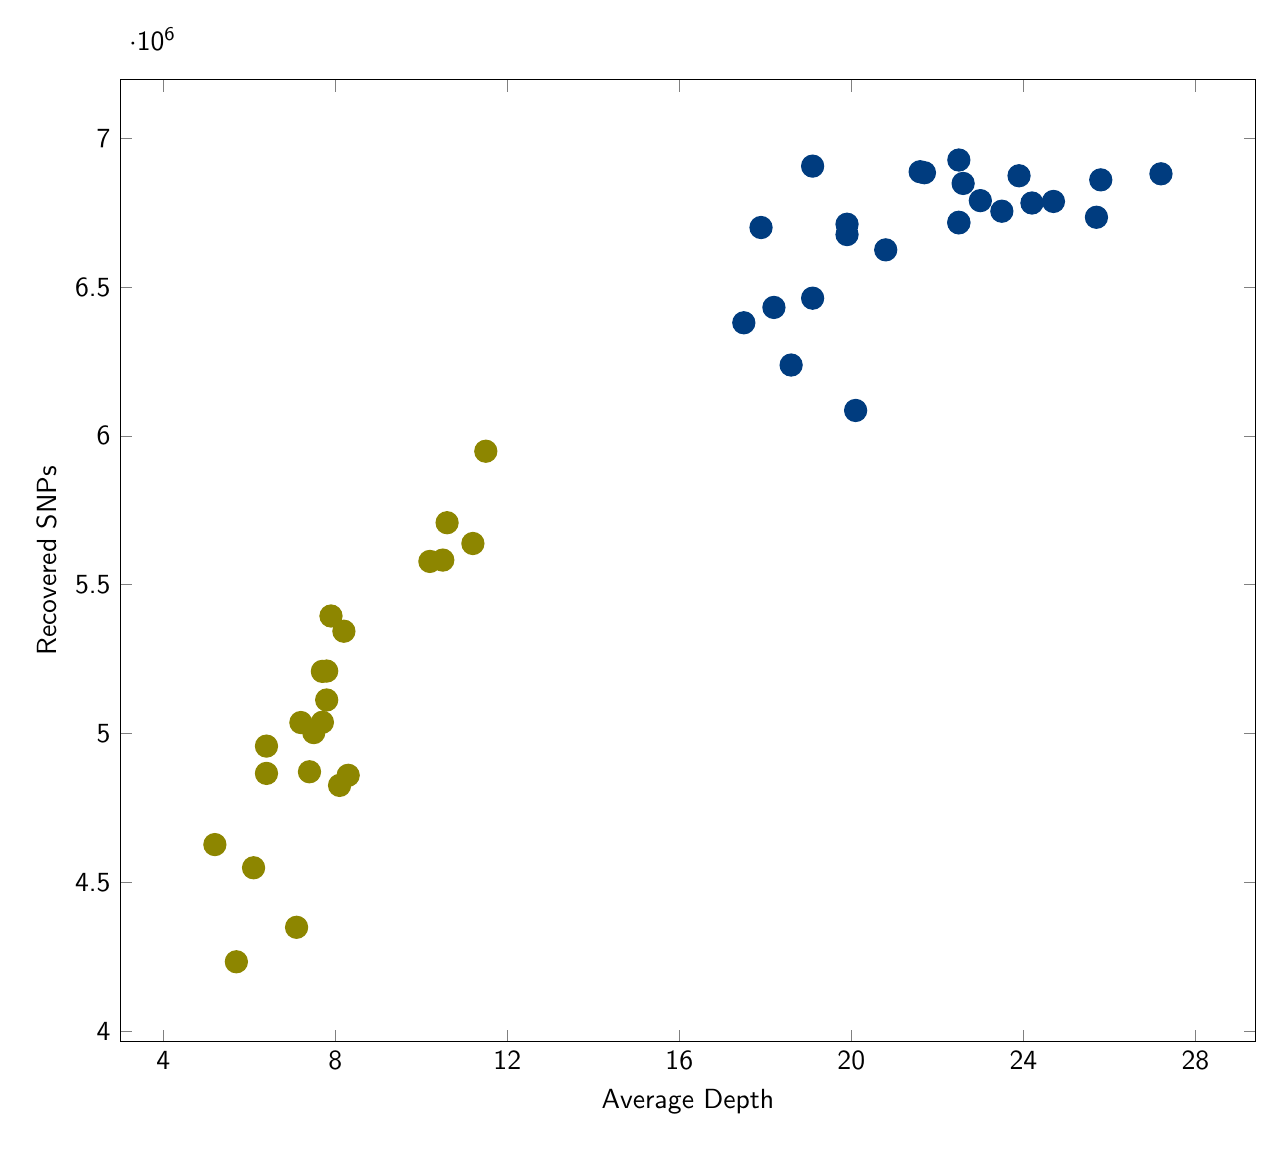
\begin{tikzpicture}
          \begin{axis}[width=16cm,xlabel=Average Depth,ylabel=Recovered SNPs, mark size=4, xtick={4,8,12,16,20,24,28}, xlabel near ticks, ylabel near ticks]
              \addplot[only marks, olive] coordinates {
                (5.2,4627116.0)
                (8.1,4825883.0)
                (8.2,5343690.0)
                (5.7,4233535.0)
                (8.3,4859808.0)
                (6.4,4957834.0)
                (11.2,5638334.0)
                (10.5,5582624.0)
                (7.8,5112786.0)
                (7.7,5208877.0)
                (10.6,5708153.0)
                (7.8,5209953.0)
                (6.1,4549233.0)
                (6.4,4866165.0)
                (7.9,5394836.0)
                (7.1,4349301.0)
                (7.2,5036978.0)
                (10.2,5578168.0)
                (7.7,5037928.0)
                (11.5,5948255.0)
                (7.4,4871668.0)
                (7.5,5003244.0)
              };
              \addplot[only marks, uoanavy] coordinates {
                (20.1,6085183.0)
                (18.6,6237718.0)
                (20.8,6624588.0)
                (17.5,6379694.0)
                (18.2,6431193.0)
                (19.9,6710671.0)
                (19.1,6462234.0)
                (21.7,6883650.0)
                (19.9,6675900.0)
                (17.9,6699604.0)
                (19.1,6905844.0)
                (21.6,6886954.0)
                (27.2,6879989.0)
                (23.5,6754383.0)
                (25.7,6734049.0)
                (24.7,6787183.0)
                (25.8,6859697.0)
                (23.0,6789875.0)
                (23.9,6873437.0)
                (24.2,6781944.0)
                (22.5,6717280.0)
                (22.5,6715159.0)
                (22.5,6926326.0)
                (22.6,6847685.0)
              };
          \end{axis}
        \end{tikzpicture}

      \end{multicols*}

    }

    \block{Overview of Methodology}{
      \begin{itemize}
        \item Want to estimate mutation and population parameters $\theta$ from \textbf{pileup data}
        \item pileup data is \textbf{unsummarized, aligned reads} for each sampled individual
        \item To compute posterior need to \textbf{marginalize over individual's genotypes}
        \item \textbf{Computationally intractable} so use \textbf{importance sampling}
        \item The importance distribution assumes independence of individual's genotypes
        \begin{align*}
          P\left(\theta \mid D \right) &= \sum_G { P\left(\theta \mid G \right) P\left(G \mid D \right) } \\
          &= \lim_{n\to\infty} \sum_{i=1}^n { P\left(\theta \mid G^{\left(i\right)} \right) \frac{P\left(G^{\left(i\right)} \mid D\right)}{\hat{P}\left(G^{\left(i\right)} \mid D \right)}}, G^{\left(i\right)} \sim \hat{P}\left(\cdot \mid D \right)
        \end{align*}
        \item Finally, use \textbf{standard MCMC to sample parameters} for a given genotype
        $$P\left(\theta \mid G \right) \propto P\left(G \mid \theta \right) P\left(\theta\right)$$
      \end{itemize}
    }

    \block{Sampling an Individual's Genotype}{
      \begin{itemize}
        \item Want the genotype $g_1, g_2 \in \left\{A, C, G, T\right\}$ of individual at a position in its genome
        \item Data is the observed base calls at this position with their Phred quality scores $$D = \left(b_q : b \in \left\{A, C, G, T\right\}, q \in \mathbb{N} \right)$$
        \item Number of base calls $\left|D\right|$ is the sequencing depth at this position
        \item Sample genotype from the posterior distribution
          $$P\left(g_1, g_2 \mid D\right) = \frac{P\left(D \mid g_1, g_2\right) P\left(g_1\right) P\left(g_2\right)}{P\left(D\right)}$$
        \item To compute $P\left(D \mid g_1, g_2\right)$ assume base calls are multinomially distributed with probabilities
          $$P\left(b_q \mid g_1, g_2 \right) = \frac{1}{2} P\left(b_q \mid g_1 \right) + \frac{1}{2} P\left(b_q \mid g_2 \right)$$
        \item Using the definition of a Phred quality score (assuming equal error rates for all bases)
        $$P\left(g_i \mid b_q \right) = \begin{cases} 1 - 10^{\frac{-q}{10}} & \mathrm{if } b = g_i \\ \frac{1}{3} 10^{\frac{-q}{10}} & \mathrm{if } b \neq g_i\end{cases}$$
        we have
        $$P\left(b_q \mid g_i \right) = \frac{P\left(g_i \mid b_q \right) P\left(b_q\right)}{P\left(g_i\right)}$$
        \item Use empirical estimates for $P\left(g_i\right)$ and $P\left(b_q\right)$
      \end{itemize}
    }

    \column{0.5}

    \block{Genotype Probability}{
      \begin{itemize}
        \item Assumes that \textbf{sites are unlinked}; i.e., phylogenetically independent
        \begin{itemize}
          \item \textbf{Models recombination} with \textbf{no dependence on correct phasing}
        \end{itemize}
        \item Assumes a site is \textbf{biallelic}; i.e., has only two possible nucleotide states
        \begin{itemize}
          \item Often true in practice
          \item Can be handled rigorously with \textbf{ascertainment bias correction}
        \end{itemize}
        \item Want the probability of all the individuals' genotypes by marginalizing over all phylogenies
          $$P\left(G \mid \theta\right) = \int_T P\left(G \mid T, \theta\right) P\left(T \mid \theta\right) \,\mathrm{d}T$$
        \item Integral is \textbf{computed numerically} using similar technique to SNAPP [2]
        \item \textbf{Divide time into intervals} using sampling times and population change times
        \item Each interval $i$ can be described by a \textbf{linear system of differential equations} $\mathbf{Q}_i$
        \item Solve each system by taking the \textbf{matrix exponential} $\exp{\mathbf{Q}_i}$ [1]
        \item \textbf{Can be done efficiently} by caching and reusing matrix exponentials
      \end{itemize}
    }

    \block{Simulation Study}{
      \begin{multicols*}{2}
        \flushleft
        \begin{itemize}
          \item 8 diploid taxa, including 4 ancient individuals up to 50k years old
          \item Mutation rate $\mu = 10^{-9}$ s/s/yr
          \item HKY model with $\kappa = 5$
          \item Constant size population with $N_e = 3 \times 10^6$
          \item Simulated 50 datasets of $10^4$ total sites
          \item Attempted to infer parameters
          \item \textbf{True values always within 95\% HPD}
          \item Mean $\hat{\mu}$ within $\pm 1.8 \times 10^{-10}$ of true $\mu$
        \end{itemize}
        \vfill
        \null
        \columnbreak
        \centering
        \includegraphics[width=16cm]{simulation.pdf}
      \end{multicols*}
    }

    \block{Summary}{
      \begin{itemize}
        \item Fully Bayesian inference of mutation and population parameters from raw sequencing data
        \item Considers both \textbf{biological processes} and \textbf{practical problems}
        \item Critically, \textbf{avoids systematic bias} due to low coverage of ancient genomes
        \item \textbf{Combats intractability} using a variety of numerical and Monte Carlo techniques
        \item Looks promising but needs \textbf{comprehensive simulation study}
        \item Applying to a very exciting dataset!
      \end{itemize}
    }

    \block{Acknowledgements}{
      \flushleft
      \begin{multicols*}{2}
        \begin{itemize}
          \item David Bryant and Remco Bouckaert
          \item Dong Xie
        \end{itemize}
      \end{multicols*}
      \begin{itemize}
        \item Sankar Subramanian, Matthew Parks, and David Lambert
      \end{itemize}
      \begin{multicols*}{2}
        \begin{itemize}
          \item New Zealand eScience Infrastructure
          \item SMBE16 Conference
        \end{itemize}
      \end{multicols*}
    }

    \block{References}{
      \flushleft
      \begin{enumerate}
      \item AH Al-Mohy and NJ Higham. \emph{SISC} 33.2 (2011). \texttt{\doi{10.1137/100788860}}
      \item D Bryant et al. \emph{Mol Biol Evol} 29.8 (2012). \texttt{\doi{10.1093/molbev/mss086}}
      \item M Li et al. \emph{Nucleic Acids Res} 32.17 (2004). \texttt{\doi{10.1093/nar/gkh850}}
      \end{enumerate}

    }

    \block{Interested?}{
      \begin{multicols*}{2}

        \flushleft

        \qrcode[height=5cm]{http://doi.org/10.5281/zenodo.56495}
        Download this poster.

        \vspace{25pt} \texttt{\doi{10.5281/zenodo.56495}}

        \columnbreak

        \qrcode[height=5cm]{http://git.io/vo7HR}
        Fork the source code.

        \vspace{25pt} \url{git.io/vo7HR}

      \end{multicols*}
    }

  \end{columns}

\end{document}